\begin{figure*}[h]
\begin{subfigure}{0.18\linewidth}
\centering
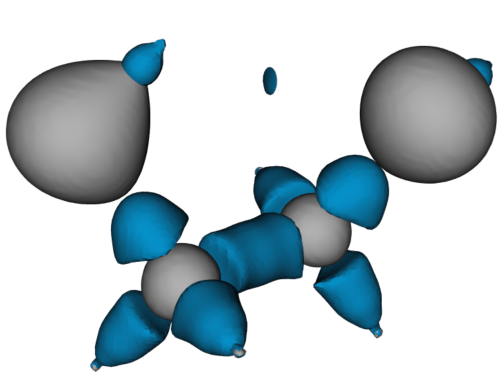
\includegraphics[width=\linewidth]{Images/EthaneDiol/gt.pdf}
\caption{$Rho_{isoval}=1.57$ (gray),\\ $s_{isoval}=-0.575$ (light blue)}
\label{}
\end{subfigure}
\begin{subfigure}{0.18\linewidth}
\centering
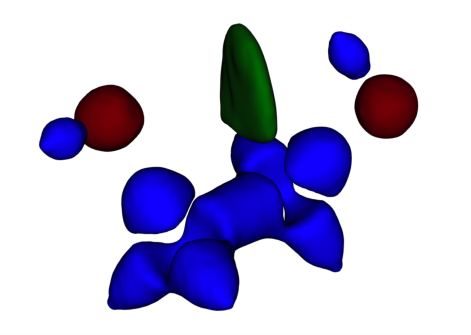
\includegraphics[width=\linewidth]{Images/EthaneDiol/zls_3.pdf}
\caption{$ZLS_{T}$}
\label{}
\end{subfigure}
\begin{subfigure}{0.18\linewidth}
\centering
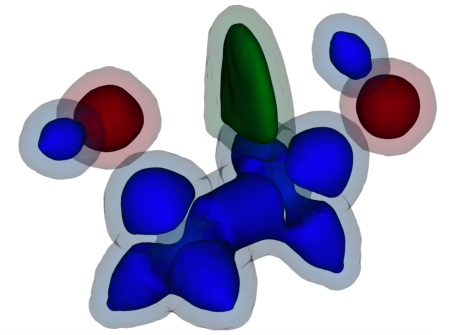
\includegraphics[width=\linewidth]{Images/EthaneDiol/fls_2_3.pdf}
\caption{$ZLS_{T}$ + $FLS_{T,2}$}
\label{}
\end{subfigure}
\begin{subfigure}{0.18\linewidth}
\centering
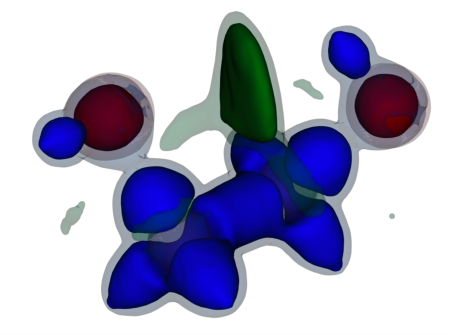
\includegraphics[width=\linewidth]{Images/EthaneDiol/fcls_68_3.pdf}
\caption{$ZLS_{T}$ + $FCLS_{T,68\%}$}
\label{}
\end{subfigure}
\begin{subfigure}{0.24\linewidth}
\centering
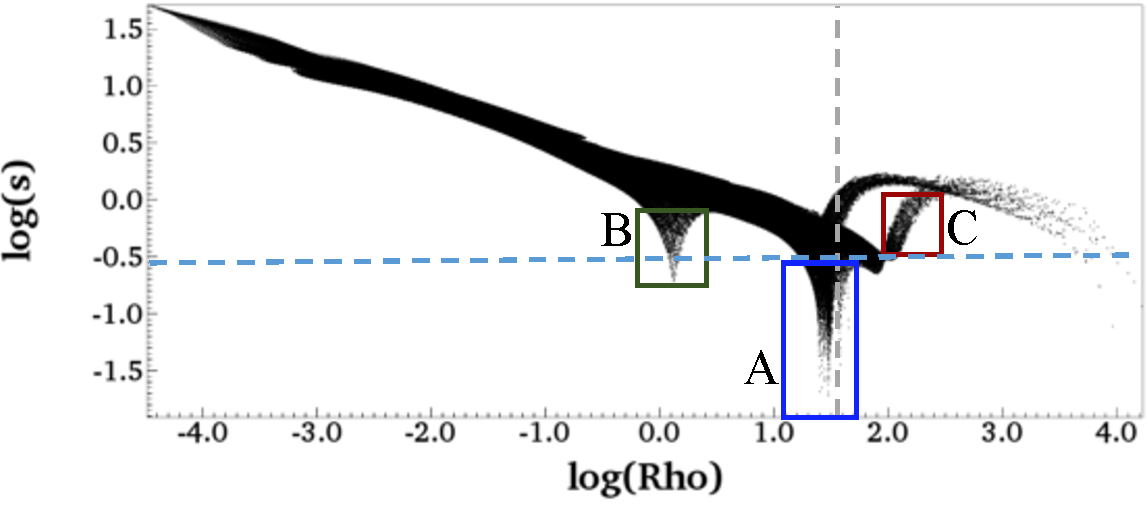
\includegraphics[width=\linewidth]{Images/EthaneDiol/scatterplot_3.pdf}
\caption{Attribute space 2D scatterplot, traits (labeled rectangular selections), and isovalues (dashed lines). We use $T = \left\{T_{A}, T_{B}, T_{C}\right\}$.} 
\label{}
\end{subfigure}
\caption{}
\label{}
\end{figure*}
